% !TeX root = ../solution.tex

\hypertarget{he22.14}{%
\chapter{[HE22.14] Snoopy}\label{he22.14}}

\begin{marginfigure}
	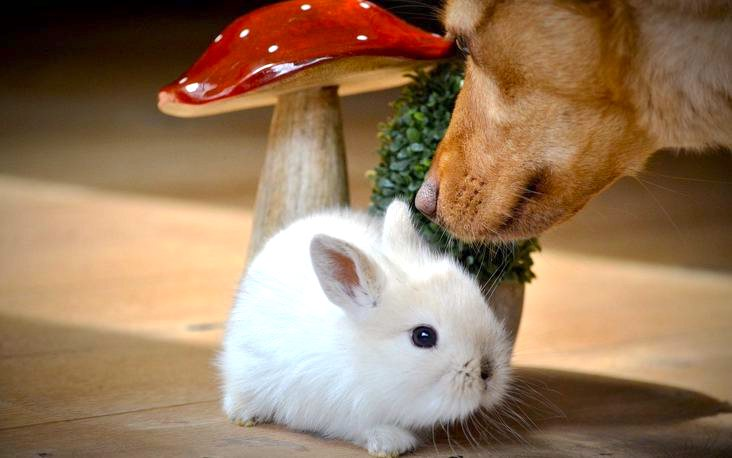
\includegraphics[width=49mm]{level4/challenge14.jpg}
\end{marginfigure}
\subsection{Intro}
Snoopy dog found something interesting.

\noindent
Can you get something interesting out of the 256 bytes he found?

\noindent\begin{verbatim}
IKIANJKDPKKAPJIDNKKAPNBHELCBHMGGDLOBLIPCKNAHFOEEBNFHALLB
OMPGKJADFKDAGMNGIIGCDPEFBINCIPNFIMKGPPLFOMLGOKFAAIECBPJF
M</Password><Domain type="NT">CORP</Domain></Credentials><ClientName>
THUMPERSDESK7</ClientName><ClientType>ica30</ClientType><ClientAddress>
10.1  
\end{verbatim}

\section{Solution}\label{hv22.14solution}
Googling for the keys in the file (<DOMAIN> etc) points us towards Citrix 
configuration files.  So the hash for the password is probably Citrix ctx1 
encoded.  \href{https://cyberchef.org/}{CyberChef} has a recipe to decode 
the password, but complains about the wrong length.  Going the other way, 
starting with a password "he2022", shows a encoded password that starts 
with "MNGIKI...", so just add "MNG" to the front of the intercepted hash to 
get
\verb+he2022{ctx1_41nt_3nKryp710n!}+.




